%   This file is part of the AIP files in the AIP distribution for REVTeX 4.
%   Version 4.1 of REVTeX, October 2009
%
%   Copyright (c) 2009 American Institute of Physics.
%
%   See the AIP README file for restrictions and more information.
%
% TeX'ing this file requires that you have AMS-LaTeX 2.0 installed
% as well as the rest of the prerequisites for REVTeX 4.1
%
% It also requires running BibTeX. The commands are as follows:
%
%  1)  latex  aipsamp
%  2)  bibtex aipsamp
%  3)  latex  aipsamp
%  4)  latex  aipsamp
%
% Use this file as a source of example code for your aip document.
% Use the file aiptemplate.tex as a template for your document.
\documentclass[%
 aip,
 jmp,%
 amsmath,amssymb,
%preprint,%
reprint,%
%author-year,%
%author-numerical,%
]{revtex4-1}

\usepackage{amsmath}  % needed for \tfrac, \bmatrix, etc.
\usepackage{amsfonts} % needed for bold Greek, Fraktur, and blackboard bold
\usepackage{graphicx} % needed for figures

%\usepackage[pdftex]{graphicx}% Include figure files
\usepackage{tabularx}
%\usepackage{bm}% bold math
\usepackage{epstopdf}
\usepackage{siunitx}
\usepackage{xcolor}
%\usepackage{booktabs}
\epstopdfsetup{outdir=./epstopds_converted/}
%\usepackage[mathlines]{lineno}% Enable numbering of text and display math
%\linenumbers\relax % Commence numbering lines
\newcommand*\circled[1]{\raisebox{0.5pt}{\textcircled{\raisebox{-.9pt} {#1}}}}
%\newcommand{\hh}{\\ \vspace{0.1cm} \\}
%\graphicspath{{D:/David/Figures/}}
\graphicspath{{epstopds_converted}}


\begin{document}

\preprint{AIP/123-QED}

\title[Sample title]{Differential Dynamics Microscopy to characterize Brownian motion and bacteria motility}% Force line breaks with \\

\author{David Germain}
\author{Mathieu Leocmach}
\author{Thomas Gibaud}
\affiliation{Universit\'e de Lyon, Laboratoire de Physique, \'Ecole Normale Sup\'erieure de Lyon, CNRS UMR 5672, 46 All\'ee d'Italie, 69364 Lyon cedex 07, France}

\date{\today}% It is always \today, today,
             %  but any date may be explicitly specified

\begin{abstract}
Abstract
\end{abstract}

\pacs{Valid PACS appear here}% PACS, the Physics and Astronomy
                             % Classification Scheme.
\keywords{Suggested keywords}%Use showkeys class option if keyword
                              %display desired
\maketitle

\begin{quotation}
``lead paragraph''
\end{quotation}

\section{\label{sec:level1}Introduction}

Quantifying the microscopic dynamics of a suspension gives access to interesting physics, both in teaching and research context. Precise measures of Brownian motion a century ago firmly proved the existence of atoms. More recently, the motion of tracer colloids has been used to extract the mechanical properties of fluids, gels, pastes, cell cytoplasm and foods, measuring viscosity or elasticity at scales unreachable by macroscopic techniques. In the past decade, the collective motion of active systems, fish schools, bird flocks and bacteria swarms has become the focus of attention of a large research community. In all these examples, one need to get access to the motion of the particles, either colloids or bacteria.

Video Particle Tracking (VPT) and Dynamic Light Scattering (DLS) are two well-known techniques. VPT consists in tracking the position of a particle as a function of time and then analyzing this trajectory. It provides precise information of small portions of a sample \citep{7_jaqaman2008robust}. DLS consists in shining a laser though the suspension and monitoring the fluctuations of scattered intensity as a function of time. It yields average information about the dynamics of a sample \citep{18_sartor2003dynamic}.




% Unlike particle tracking, it works in the Fourier space. Applying those two methods simultaneously would allow a powerful combination of their complementary informations but it is not easy to apply as they are based on two different process. In VPT, a direct capture of the sample through a microscope is needed whereas DLS is based on the measure of the scattering angle to get the spatial wave vectors of the sample. To do so, the many attempts which has been done implied the customization of a microscope \citep{27_kaplan1999light, 28_valentine2001microscope, 29_dzakpasu2004dynamic} (Laser light source, suitable lens to obtain the Fourier transform of the sample optically, several hardware to do both the calculation for the VPT and the DLS, ...). The difficulties to build such an equipment limit the number of laboratories which could do such experiments.

 

Here, we describe an alternative method call Differential Dynamic Microscopy (DDM) recently proposed by XXX. DDM uses a standard light microscope linked to a camera and relies on digital Fourier transform to obtain the same kind of information as DLS, but with some of the spatial resolution of VPT. In a teaching context, since DDM starts with a real-space video of the moving objects it is less abstract than DLS. The explicit use of Fourier transform may also help to demystify this operation that is at the cornerstone of modern physics. 

In this article, we will apply DDM to two sets of different micrometric particles, colloids at first, then motile bacteria. In a first part, we will present the materials and method we used to prepare the samples as well as the acquisition parameters. Then we will use the Brownian motion as a support to a step by step presentation of the DDM in a fully understood context. In a last part, we will apply DDM to bacteria of the species \textit{salmonella} and show that it is possible to obtain the Brownian diffusion coefficient, but also the mean speed of run, the rate of motile bacteria, and a preview XXX of the velocity distribution.

\section{Materials and method}

%We capture a stack of images of aqueous dispersions of colloids or bacteria observed under a microscope.

\subsection{Colloidal particles}

Colloids are FluoSpheres\circledR{} from Thermo Fisher Scientific. They are spheres made of polystyrene of density $\rho_\text{coll} = \SI{1.06}{\gram\per\litre}$ and have a catalog diameter of $d = \SI{1.0}{\micro\meter}$. The commercial dispersion is diluted 50 times in water to a final concentration of $\SI{1e8}{colloids\per\milli\liter}$ so that we have a dilute dispersion: the distance between two colloids is large compared to $d$, typically $10 d$. This concentration remains sufficiently high to observe enough particles in the camera field of view and to accumulate decent statistics.

Polystyrene refractive index is $\approx 1.6$, larger than the one of water $\approx 1.3$, so the colloids are visible by usual light microscopy. However cleaner images can be obtained by fluorescence microscopy, exiting at \SI{540}{\nano\metre} and filtering to obtain the emmited light at \SI{560}{\nano\metre}.

%The size of a water molecule (H$_2$O) $\simeq \SI{0.34}{\nano\meter}$, which is far smaller than the size of a sphere, so, we are in colloidal regime. Also, during our acquisitions, sedimentation is negligible, $Pe_\text{g} \gg 1$.
%We also checked afterwards directly on the acquisitions. If there were sedimentation, we would lose the focus on colloids. Also, we checked if there were a flow in the microscope slide by looking at the motion of colloids. If there were a flow, the average motion of colloids would be in the direction of this flow instead of being equal to zero.

\subsection{Bacteria}

In section \ref{sec:BactSection}, we study the motion of \textit{Salmonella} bacteria (DSM. 1103) \citep{21_fabrega2013salmonella}. Our bacteria are stored in a freezer at $\SI{-80}{\degree C}$ in a mixture of water ($\simeq \SI{33}{\%}$) and glycerol ($\simeq \SI{66}{\%}$). First, using a sterile inoculation loop, we take a small volume of this storage solution  and we spread it on a sterile Petri dish filled with a mixture of agar and LB ($\SI{500}{\milli\liter}$ of LB/agar was made of $\SI{5}{\gram}$ of NaCl, $\SI{5}{\gram}$ of Tryptone, $\SI{2.5}{\gram}$ of Yeast Extract, $\SI{7.5}{\gram}$ of Agar and water up to $\SI{500}{\milli\liter}$). We start from one side of the dish, then we make a zig-zag trajectory with the inoculation loop being careful there is no crossing. Then we take another loop, and we start a new trajectory from the end of the previous one. Second, the agar plates are closed and placed in an incubator at $\SI{37}{\degree C}$. The agar plates are oriented such that the LB/agar gel is at the top, to prevent the condensation from disturbing the development of the bacteria. After $\simeq$ 12 hours, we observe the formation of monoclonal circular colonies. Third, Using \textcolor{red}{(an ?)} inoculation loop, we take a monoclonal colony of bacteria from LB/Agar plate and disperse it in a \textsc{Falcon} tube with $\simeq \SI{5}{\milli\liter}$ TN growth medium. The TN growth medium is sterile and composed of $\SI{4}{\gram\per\liter}$ of bacto-tryptone, $\SI{2.5}{\gram\per\liter}$ of NaCl and $0.4\%$ of glycerol diluted in water. The \textsc{Falcon} tubes have an oxygen permeable cap which allows the bacteria to breath and limits evaporation. Those bacteria are pre-cultured for a night at $\SI{32}{\degree C}$ and shaked at 300 rpm in an Incu-Shaker 10L. Finally, we collected $\SI{50}{\micro\liter}$ of the solution of bacteria with a sterile pipette and we put it in a new \textsc{Falcon} tube filled with $\simeq \SI{5}{\milli\liter}$ of TN growth medium. The tube is then placed in the Incu-Shaker 10L at 300 rpm and $\SI{32}{\degree C}$ for 1h30. Around this time the optical density at $\SI{600}{\nano\meter}$ is around OD=0.5 and most bacteria are swimming. It is important to grow bacteria in a nutriment poor media and to collect them early on, at low concentrations, otherwise the bacteria tend not to develop a flagella.

\subsection{Microscope slide}
For the microscope observations, the aqueous suspension of colloids or bacteria are enclosed in a hermetic microscope slide (FIG. \ref{Slide}). The  slide is composed of a  glass slide (\textsc{RS France}) and a cover slip (\textsc{Menszel-gl\"aser}) spaced by two lamellas of parafilm (\textsc{Bemis}).  The space between the glass slide and the cover slip is approximately $\SI{125}{\micro\meter}$.  The slide is then heated on a hotplate for 5 minutes to melt the parafilm thus sticking the cover slip and the glass slide together. A suspension of colloids or bacteria is then introduced into the enclosure by capillarity. Finally, the sample is sealed by application of glue (\textsc{Norland Products}) which hardens in contact of UV light ($\lambda = \SI{365}{\nano\meter}$).


\begin{figure}
\includegraphics[width=\linewidth]{Colloides/ModifiedInkscape/Lamelle.eps}
\caption{Skematics of the microscope slide used to study the motion of particles, namely, colloids and bacteria).}
\label{Slide}
\end{figure}

\subsection{Microscope and acquisition parameters}

The colloidal suspension is observed with light microscope (\textsc{nikon Eclipse Ti}) in visible light with an objective $10 \times$ and a numerical aperture $N.A. = 0.3$. The focus is made in the middle of the microscope slide in z-direction. It allows to be far from the boundaries where colloids could be stuck on the slide and could not move in the 3 dimensions. Image are acquired with a camera (\textsc{Hamamatsu digital camera C11440}).

The images are coded in $\SI{8}{bits}$  grey-scale: each pixel intensity is proportional to the incoming light intensity from the sample and varies linearly from  0 (black) to 255 (white). Using an exposure time of $\SI{1}{\milli\second}$, we adjusted the brightness of the microscope light in order to have a maximum number of pixel around a value of $\sim 120$ which minimize the amount of saturated pixels.

The choice of the acquisitions parameters is a compromise between the spatial resolution and the temporal resolution. With the $10\times$ objective, a pixel correspond to $\SI{0.645}{\micro\meter}$, roughly the optical resolution of the microscope. A bacteria or the colloids is about $\SI{1}{\micro\meter}$ and therefore correspond to a few pixels on the camera. We chose a $512 \times 512$ px$^2$ field of view which is large enough to capture the motion of 100 of bacteria and small enough so that we may have a high acquisition frequency, up to $\SI{400}{\hertz}$.

By looking at the videos of colloids and bacteria, we see that the dynamics happens on the time scale of $\SI{1}{\second}$. We therefore chose to acquire a first stack of 4000 images of  $512 \times 512$ px$^2$ at $\SI{400}{\hertz}$ and a second similar stack at $\SI{4}{\hertz}$. The stack size, 4000 images, is limited by the camera buffer memory. At $\SI{400}{\hertz}$ it is impossible to directly sent the data from the camera to the computer during the capture, so we chose to temporarily save the acquisition on the buffer of the camera during the capture, and, once it is over, we send the data from the buffer of the camera to the computer. With this procedure, the smallest time scale is $\SI{2.5e-3}{\second}$ and the largest is $\SI{1000}{\second}$ and the smallest length scale is $\SI{0.645}{\micro\meter}$ micron and the largest is $\SI{330}{\micro\meter}$. 



\section{Brownian motion and DDM}
\label{sec:BrownSection}

\subsection{The Brownian motion}

The Brownian motion is the unceasing and random motion of small particles in suspension in a liquid at rest. Brownian motion has a particularly interesting history. It has been observed since the 18th century, and maybe even before. Robert Brown, a Scottish botanist from the beginning of the 19th century, who was interested in the action of pollen on plant reproduction, observed the irregular and unceasing motion of micrometric particles in the internal fluid of grain of pollen \citep{13_brown1828brief}. At the time, such microscopic agitation was seen as \textit{a priori} a vital phenomenon. Nevertheless, R. Brown showed that this phenomenon persist with inorganic particles, refuting the wrong concept based on living particles. It's only at the beginning of the 20th century that physicists could interpret and analyse the Brownian motion. \textcolor{red}{XXX?} What is particular with Brownian motion and has prevented every attempt of interpretation in the 19th century, is that this motion is perpetual, unlike other usual experiments where friction eventually stop the motion. Albert Einstein \citep{9_einstein1906theory}, William Sutherland \citep{14_sutherland1905lxxv}, Marian von Smoluchowski \citep{10_von1906kinetischen} and Paul Langevin \citep{15_Langevin} rely on the molecular assumption, the thermostatically-controlled fluid containing the Brownian particles is composed of molecules which size is far smaller than the Brownian particles. They demonstrated that it is the shocks between the molecules of the liquid and the Brownian particles that are at the origin of the Brownian motion. This assumption has been validated by the experiments made by Jean Perrin in 1928 \citep{22_perrin2014atomes}. With a microscope and photographs, the team of Jean Perrin reconstructed ``by hand" the trajectories of Brownian particles and deduced a correct measure of the Avogadro constant, validating the theory of Brownian motion.

\subsection{Colloidal particles}

To observe the Brownian motion of a particle in a Newtonian fluid, several conditions are required \citep{16_CollSusp}. The particle has to be colloidal, meaning that its size has to be far larger than the size of the molecule of the solvent, it is the case for the suspension we used (Table \ref{TabParams}). Furthermore, colloidal particles have to be in dilute regime to avoid interaction between them. This is checked once the sample is made. As our colloids do not have long distance interaction, we estimate that the sample is dilute when the mean distance between colloids is higher than at least 10 times the diameter of a colloid. Finally, one has to make sure that the thermal agitation is the physical process that dominate the dynamic of the colloidal particle. We ensure that the solvent is not flowing by using an immobile, sealed and thin optical cell with negligible temperature gradient. The sedimentation motion can be characterized by the P\'eclet number \citep{12_patankar1980numerical}
\begin{equation}
\text{Pe}_g = \frac{E_g}{E_\text{th}},
\end{equation}
where $E_g = \frac{\pi d^3}{6}  (\rho_\text{c} - \rho_\text{s}) g  d$ is the variation of potential energy for a difference of altitude equal to the diameter $d$ of the particle, $E_\text{th} = k_\text{B} T$ is the thermal energy, $\rho_\text{c}$ and $\rho_\text{s}$ the respective densities of the particle and the surrounding solution, $g$ the acceleration of gravity, $k_\text{B}$ the Boltzmann constant and $T$ the temperature. Here $\text{Pe}_g \approx 0.1$, indicating that the sedimentation can be neglected over Brownian motion, at least when the particles have moved by less than a diameter during the acquisition time.


Absence of both flow and sedimentation will be verified \textit{a posteriori}. In presence of a flow the trajectory of the colloid, normally random, is biased in the direction of the flow. In presence of gravitational effects, the colloids sediment in the z-direction and the focus made with the microscope on the colloid is lost. 

\begin{table}
\begin{tabular}{m{0.7\linewidth}m{0.28\linewidth}}
  \hline\\[-0.8em]
  Molecular diameter of water \citep{17_marcus1998properties}  & $\SI{0.34}{\nano\meter}$\\
  Temperature $T$ of the suspension & $\SI{20}{\degree C}$ \\
  Tabulated viscosity of water at $T$ & $\SI{1.002}{\milli\pascal\second}$ \\
  Density of polystyrene & $\SI{1.04}{\gram\per\centi\meter\cubed}$ \\
  Colloid diameter $2r$ & $\SI{1}{\micro\meter}$\\
  \hline
  \end{tabular}
  \caption{Properties of colloidal particles and their medium}
  \label{TabParams}
\end{table}


\subsection{Stokes-Einstein relation}

The average position $\langle X(t) \rangle$ of a Brownian particle is not a good parameter to characterize the Brownian motion. Indeed, as its motion is random with the same probability to move in any direction after a collision, $\langle X(t) \rangle \underset{t\to +\infty}{\longrightarrow} 0$ (FIG. \ref{BrownianTrajectory}.a). The mean square displacement \citep{11_ken2003molecular} $\langle X^2(t) \rangle$ is a much better parameter to computer from the trajectory of the colloid. By resolving the equation of diffusion for a density $\rho(\vec{X}, t)$ of Brownian particle, it can be shown that the second moment of $\rho(\vec{X}, t)$ is:

\begin{equation}
\langle X^2(t) \rangle = 2dDt
\end{equation}

$d$ is the dimension of the space, $D$ is the diffusion coefficient. As predicted by theory, experiments shows that the mean square displacement scales linearly with time, Fig. \ref{BrownianTrajectory}.b.

\begin{figure}
	\includegraphics[width=\linewidth]{Colloides/MatlabDirect/MouvementBrownien.eps}\\
	\includegraphics[width=\linewidth]{Colloides/MatlabDirect/MSDBrownian.eps}
	\caption{(a) Trajectory of a brownian particle obtained by particle tracking as a function of time. Positions of a colloid of diameter 1 $\mu$m in an aqueous suspension at various times from $t=0$ s (blue) to $t=2.5$ s (red). The time increment is $2.5 \times 10^{-3}$ s. (b) Mean Square Displacement of the colloid as a function of $t$ calculate from the trajectory in (a). }
	\label{BrownianTrajectory}
\end{figure}

$D$ is increasing with the temperature and decreasing with the radius $r$ of the particle and the viscosity $\eta$ of the fluid according to the \textsc{Stokes-Einstein} formula \citep{9_einstein1906theory}:

\begin{equation}
D = \frac{k_\text{B} T}{6 \pi \eta r}
\end{equation}


\subsection{Differential Dynamics Microscopy}

Just as Dynamic Light Scattering (DLS) \citep{18_sartor2003dynamic}, the DDM yields average informations about a sample dynamics in the Fourier space. In DLS we measure the intensity as a function of time scattered by the sample directly in the Fourier space whereas in  DDM, we numerically Fourier transforms the images of the sample as a function of time \citep{2_DDM}. In both cases, we obtain the intermediate scattering function (ISF), $f$, a correlation function. We can get quantitative informations about the dynamic of the sample either by scaling the correlation function or by fitting the correlation with a model.

To qualitatively get a feeling of the ISF, in FIG. \ref{SketchCorrelation}, we have superimposed two images of a colloidal dispersion separated by a lag time $\Delta t$. At $\Delta t = \SI{0.01}{\second}$, the colloids have barely moved and $f \simeq 1$. At $\Delta t = \SI{1}{\second}$, the colloids have moved and we can identity where they have come from.  At $\Delta t = \SI{100}{\second}$, the colloids have moved so much that we no longer know where they have come from and $f \simeq 0$: the 2 images are totally decorrelated.


\begin{figure}
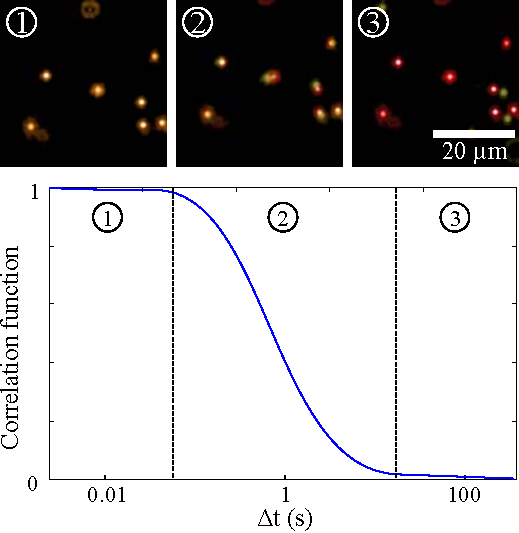
\includegraphics[width=\linewidth]{Colloides/ModifiedInkscape/ComparaisonImage.eps}
\caption{Differential Dynamic Microscopy (DDM) principle. Superpositions of 2 images of a colloidal dispersion taken at various intervals of time and sketch of the correlation function. Each picture is composed of 2 images, the first one is colored in yellow and taken at $t = 0$ s, the other is colored in red and taken at $t = \Delta t$. \protect\circled{1}: $\Delta t = 0.01$ s; \protect\circled{2}: $\Delta t = 1$ s; \protect\circled{3}: $\Delta t = 100$ s. Correlation function between 2 sets of positions associated with each pictures. At low $\Delta t$, the 2 sets are very correlated \protect\circled{1} and the correlation function is 1. For $\Delta t \sim 1$ s, the correlation decrease \protect\circled{2}. For long $\Delta t$, the 2 sets are almost completely decorrelated \protect\circled{3} and the correlation function is 0.}
\label{SketchCorrelation}
\end{figure}

The correlation function $F(\vec{q}, \, \Delta t)$ and the normalized correlation function $f(\vec{q}, \, \Delta t)$ are defined as \citep{19_goodman2005introduction} :

\begin{eqnarray}
F(\vec{q}, \, \Delta t) &=& \langle \ \hat{I}^*(\vec{q},\, t) \hat{I}(\vec{q},\, t+\Delta t) \ \rangle \\
f(\vec{q}, \, \Delta t) &=& \frac{F(\vec{q}, \, \Delta t)}{F(\vec{q}, \, 0)}
\end{eqnarray}

where $\hat{I}(\vec{q}, \, t)$ is the scattered intensity in DLS and the fourier transform of the image ${I(\vec{r} \, t}$ in DDM; $\vec{q}$ is the scattering wave vector in DLS and the Fourier vector associated to vector position $\vec{r}$ in DDM. $\langle \cdot \rangle$ is the average over $t$.

The ISF  is directly measured from $\hat{I}(\vec{q}, \, t)$ in DLS and from $\langle \, | \widehat{\Delta I}(\vec{q},\,\Delta t)|^2 \, \rangle$ with $\Delta I(\vec{q},\,\Delta t) = I(\vec{q},\, t+\Delta t) - I(\vec{q},\, t)$, in DDM:

\begin{eqnarray}
\langle \, |\widehat{\Delta I}|^2 \, \rangle &=& \langle \, |\widehat{I}(\vec{q},t+\Delta t) - \widehat{I}(\vec{q},t)|^2 \, \rangle \\ \nonumber
&=& \langle \, |\widehat{I}(\vec{q},t+ \Delta t)|^2 + |\widehat{I}(\vec{q},t)|^2 \\ \nonumber
&& \qquad \quad - 2 \, \widehat{I}^*(\vec{q},t+\Delta t) \widehat{I}(\vec{q},t) \, \rangle\\\nonumber
&=& \underbrace{2F(\vec{q}, 0)}_{\equiv A(\vec{q})} \bigg[ 1-\underbrace{\frac{F(\vec{q}, \Delta t)}{F(\vec{q}, 0)}}_{f(\vec{q}, \Delta t)} \bigg]\\\nonumber
\end{eqnarray}

The contribution of the noise due to the camera is taken into account by adding a supplementary term $B(\vec{q})$. $B(\vec{q})$ is decorrelated  at all time and therefore independent of $\Delta t$.

\begin{eqnarray}
\langle \, |\widehat{\Delta I}|^2 \, \rangle = A(\vec{q})[1-f(\vec{q}, \Delta t)] + B(\vec{q})
\end{eqnarray}

The parameters $A(\vec{q})$ and $B(\vec{q})$ can be used as fitting parameters or measured independently thus giving access directly to the ISF. For both colloids and bacteria, the samples we study are both homogeneous and isotropic, which means that we don't lose information by studying $q \equiv |\vec{q}| = \sqrt{q_x^2 + q_y ^2}$. To convert our pictures depending on $q_x$ and $q_y$ into a function depending on $q$, we realise a radial averages centred on the middle of the FFT image. The range of accessible $q$ depends on both the image and pixel size.

We note that the calculation time necessary to realize all the FFT of images at all the accessible $\Delta t$ can become very long (some hours). To \textcolor{red}{circonvint} this issue we sampled $\Delta t$ logarithmically with 10 points per decades.  Also, we didn't average over all the $|\widehat{\Delta I}|^2$ at constant $\Delta t$. We reduced the average on the first 100 differences of images which is sufficient to have isotropic Fourier transforms. With those optimizations, the calculation time fell to some minutes. We ran the DDM procedure on the both stacks of images at $\SI{400}{\hertz}$ and $\SI{4}{\hertz}$ independently. Then the we merged the two sets of data by multiplying each value of $|\widehat{\Delta I}|^2$ obtained at $\SI{4}{\hertz}$ so that $|\widehat{\Delta I}(q,\Delta t = \SI{0.25}{\second})|^2_{\SI{4}{\hertz}}$=$|\widehat{\Delta I}(q,\Delta t = \SI{0.25}{\second})|^2_{\SI{400}{\hertz}}$. Finally, we average the values of the curves at $\SI{4}{\hertz}$ and $\SI{400}{\hertz}$ in the overlap interval, from $\SI{0.25}{\second}$ to $\SI{10}{\second}$). We obtain $\langle \, |\widehat{\Delta I}|^2 \, \rangle (q, \Delta t)$ for $\Delta t$ from $\SI{2.5e-3}{\second}$ to $\SI{1000}{\second}$. The DDM procedure is summarized in Table \ref{AlgoTable}.

\begin{table}
\begin{tabular}{ |p{0.98\linewidth}| }
  \hline
  \\  
  Two acquisitions:
  \begin{itemize}
  \item 4000 images $I(\vec{x},t)$ per acquisitions
  \item Acquisiton 1 : $f=\SI{400}{\hertz} \rightarrow t_\text{max} = \SI{10}{\second}$
  \item Acquisiton 2 : $f=\SI{4}{\hertz} \rightarrow t_\text{max} = \SI{1000}{\second}$
  \item Exposition time = $\SI{1}{\milli\second}$
  \item Resolution of images = $512\times\SI{512}{px^2}$
  \end{itemize}
  \\
  \hline
  \\
  DDM algorithm:\\[2ex]
  \hspace{0.3cm} for $\Delta t = 1/f \rightarrow t_\text{max}$ in log scale: \\[1ex]
  \hspace{0.6cm} for $t = 0 \rightarrow \text{max}(t_\text{max}- \Delta t$ or $100)$: \\
  \hspace{0.9cm} $\Delta I(\vec{x},t,\Delta t) = I(\vec{x},t+\Delta t) - I(\vec{x},t)$\\
  \hspace{0.9cm} $|\widehat{\Delta I}(\vec{q},t,\Delta t)|^2 = |\text{FFT}[\Delta I(\vec{x},t,\Delta t)]|^2$\\
  \hspace{0.6cm} end\\[1ex]
  \hspace{0.6cm} Average on time $\rightarrow \langle \, |\widehat{\Delta I}|^2 \, \rangle (\vec{q}, \Delta t)$\\
  \hspace{0.3cm} end\\[1ex]
  \hspace{0.3cm} Radial average $\rightarrow \langle \, |\widehat{\Delta I}|^2 \, \rangle (q, \Delta t)$\\
  \\
  \hline\\
  Fit of $\langle \, |\widehat{\Delta I}|^2 \, \rangle$:\\[2ex]
  \hspace{0.3cm} $\langle \, \widehat{|\Delta I}|^2 \, \rangle (q, \Delta t) = A(q)(1-\underbrace{f(q, \Delta t)}_\text{ISF})+B(q)$ \\
  \\
  \hline\\
  Scales:
  \begin{itemize}
  \item $\SI{1}{px} = \SI{0.645}{\micro\meter}$
  \item $q_\text{min} = \frac{2 \pi}{0.645 \times 512} = \SI{1.9e-2}{\per\micro\meter}$
  \item $q_\text{max} = \frac{2 \pi}{0.645 \times 512} 256 = \SI{4.9}{\per\micro\meter}$
  \end{itemize}\\
  \hline
\end{tabular}
\caption{table}{Steps of application of DDM}
\label{AlgoTable}
\end{table}


\subsection{Results}

We first apply DDM on a suspension of colloids. In FIG. \ref{DifferenceAndFFT} we show $I(\vec{r}, \, t)- I(\vec{r}, \, t+\Delta t)$ for increasing value of $\Delta t$ and the corresponding power spectrum of each images. As $\Delta t$ increases, colloids move more and the difference between two images shows a growing signal on larger and larger length scale. \textcolor{red}{In FIG. \ref{D}.a, we have plotted the corresponding power spectrum.} The power spectrum is isotrope and as $\Delta t$ increases a peak appears at a wave vector which correspond to the most probable distance between two colloids. 

\begin{figure}
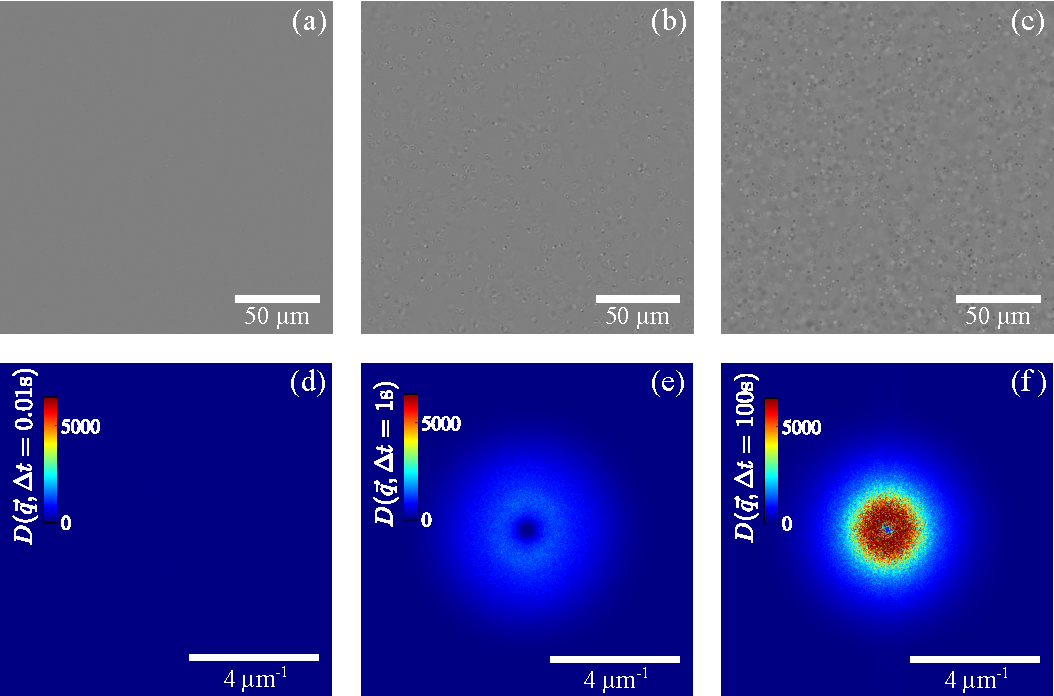
\includegraphics[width=\linewidth]{Colloides/ModifiedInkscape/Diff_TF.eps}
\caption{Image differences of a colloidal suspension and their Fourier transform as a function of $\Delta t$. (a, b, c) Differences between 2 images separated by $\Delta t$. (d, e, f) 2D Fourier transforms of those differences. These differences and Fourier transforms are calculated with $\Delta t = 0.01$ s (a, d), $\Delta t = 1$ s (b, e), $\Delta t = 100$ s (c, f). The unit of the Fourier transforms is arbitrary.}
\label{DifferenceAndFFT}
\end{figure}


in FIG. \ref{D}, $\widehat{\Delta I}(\vec{q}, \Delta t)$ is plotted as a function of $q$ and $\Delta t$. For small $\Delta t$ (FIG. \ref{D}.b), we observe a first plateau. Images are very correlated, colloids didn't move enough between 2 acquisitions separated by $\Delta t$ and the colloids motion is barely visible on the differences between the images. Thus, $f(\vec{q}, \, \Delta t) \simeq 1$,  we only observe the contribution of the noise $B(q)$. For large $\Delta t$, we observe a second plateau at a higher value because the images are completely decorrelated, $f(\vec{q}, \, \Delta t) \simeq 0 \rightarrow \langle \, |\widehat{\Delta I}|^2 \, \rangle (q, \, \Delta t) \simeq A(q)+B(q)$. The decorrelation appears faster when $q$ increases. Large $q$ correspond to small objects, considering a constant speed for objects at every scales, small objects decorrelate faster than big ones (corresponding to small $q$).

\begin{figure}
	\includegraphics[width=\linewidth]{Colloides/MatlabDirect/MoyenneRadialeSpline.eps}\\
	\includegraphics[width=\linewidth]{Colloides/MatlabDirect/Dexpe.eps}
	\caption{Evolution of the Fourier transforms $\langle \, |\widehat{\Delta I}|^2 \, \rangle (q, \Delta t)$ of the differences of images as a function of the the wave vector $q$ calculated at various $\Delta t$ (a) and as a function of $\Delta t$ calculated at various $q$ (b).}
	\label{D}
\end{figure}

For a stochastic process such as the Brownian motion, the decrease of the correlation function is exponential : $ f(q, \, \Delta t) = \exp(-\frac{\Delta t}{\tau_\text{d}})$, with $\tau_\text{d}$ the characteristic time of the decay \citep{8_berne2000dynamic}. We fitted $\langle \, |\widehat{\Delta I}|^2 \, \rangle (q, \Delta t)$ as a function of $\Delta t$ for fixed $q$ and for each $q$. Our fit parameters are $A(q)$, $B(q)$ and $\tau_\text{d}(q)$. We fit the data in logarithmic scale in order not to attribute to much weight on points with high intensity. The initial parameters for the fit are:

\begin{equation}
\left\{
\begin{array}{rcl}
A_0 &=& \langle \, |\widehat{\Delta I}|^2 \, \rangle (q,\Delta t_\text{max}) - \langle \, |\widehat{\Delta I}|^2 \, \rangle (q,\Delta t_\text{min}) \\
B_0 &=& \langle \, |\widehat{\Delta I}|^2 \, \rangle (q,\Delta t_\text{min}) \\
\tau_\text{d} &=& \SI{1}{\second}
\end{array}
\right.
\end{equation}

\textcolor{red}{where $\Delta t_\text{max}$ is the maximum interval of time between 2 images ($ = \SI{999.75}{\second}$) and $\Delta t_\text{min}$ is the minimum interval of time between 2 pictures ($ = \SI{2.5e-3}{\second}$).}

where $\Delta t_\text{max}$ and $\Delta t_\text{min}$ are respectively the maximum and the minimum interval of time between two images.

Using the fit results for $A(q)$ and $B(q)$, we obtain the ISF (FIG. \ref{ISF}.a). It is possible to model $\tau_\text{d}$. For Brownian motion, $\tau_\text{d}$ is the characteristic time necessary for the colloid to travel a distance $L$. In real space, this results is $\tau_\text{d} = \frac{L^2}{D_\text{coll}}$ and in Fourier space, $\tau_\text{d} = \frac{1}{D_\text{coll} q^2}$ with $D_\text{coll}$ the diffusion coefficient due to Brownian motion for our colloids. By plotting $f(q, \Delta t)$ as a function of $\Delta t q^2$, we remove every dependence of the ISF on $q$ resulting into a collapse of the data on a master curve. (FIG. \ref{ISF}.b). 

\begin{figure}
	\includegraphics[width=\linewidth]{Colloides/MatlabDirect/ISF+Fit_t.eps}\\
	\includegraphics[width=\linewidth]{Colloides/MatlabDirect/ISF+Fit_tq2.eps}
	\caption{Intermediate scattering function (ISF) calculated at various $q$ versus $\Delta t$ (a) and $\Delta tq^2$ (b).}
	\label{ISF}
\end{figure}

When plotting $\tau_\text{d}(q)$ as a function of $q$ (FIG. \ref{FitDiffColl}.a), 3 regimes are visible:

\begin{itemize}
\item[\textbf{(1)}] The radial average is perform on very few points (1 point for $q = q_\text{min}$ which correspond to the center of the Fourier transforms). We are also limited to duration of the experiment, $\SI{1000}{\second}$.
\item[\textbf{(3)}] The signal-to-noise ratio is too high.
\item[\textbf{(2)}] Statistics are good and the signal-to-noise ratio is low enough.
\end{itemize}


Given the diffusive origin of $\tau_\text{d}$, we have fitted $\log(\tau_\text{d})$ as a function of $q$ in the regime (2) with a linear function in logarithmic scale : $\tau_\text{fit}(q) = -2\log(q) - \log(D_\text{fit})$. 



The theoretical model is in a very good agreement with our measurements and we obtain a diffusion coefficient of $D_\text{fit} = \SI{0.39}{\micro\meter\squared\per\second}$. Using the Stokes-Einstein formula with our experimental conditions $T = \SI{293}{\kelvin}$, $\eta = \SI{1}{\milli\pascal\second}$, $r = \SI{0.5}{\micro\meter}$, we obtain $D_\text{E} = \SI{0.41}{\micro\meter\squared\per\second}$ which implies an error of only $\sim 4.9 \%$. The range of $q$ on which we are able to fit $\tau_\text{d}$ provide us an experimental value for the resolution of DDM. Indeed, as the relevant regime has a maximum of $q=\SI{3.5}{\per\micro\meter}$, we obtain a resolution of $\frac{2\pi}{3.5} = \SI{1.8}{\micro\meter}$. Comparing to the microscope resolution $d = \frac{\lambda}{2 N.A.} \sim \SI{1}{\micro\meter}$, it means that the resolution of the microscope is not the limiting factor for the resolution of the DDM.

We also have access to informations about the parameters $A(q)$ and $B(q)$ (FIG. \ref{FitDiffColl}.b). According to our data, the noise floor $B(q)$ seems constant for every $q$: the camera is adding a white noise to each images. Also, it is possible to relate the parameter $A(q)$, \textcolor{red}{XXX} which is twice the autocorrelation of the studied system, to characteristics of the microscope \citep{3_DDM3D}. F.Giavazzi et al. has shown that it is related to the properties of the light source, the numerical aperture of the objective and the sample thickness.

\begin{figure}
	%\hspace{-1.5mm}
	\includegraphics[width=\linewidth]{Colloides/MatlabDirect/FitDiffusion.eps}\\
	\includegraphics[width=\linewidth]{Colloides/MatlabDirect/A+B+FitLOG.eps}
	\caption{Caracteristic brownian diffusion time and fit parameters A(q), B(q).(a) Experimental data (\textcolor{blue}{$\circ$}) and fitted curve (\textcolor{red}{\textbf{---}}) of the caracteristic time for brownian diffusion $\tau_\text{d}$ versus $q$. (b) Fit parameters A(q) ($\ast$), B(q) (\textcolor{blue}{+}), and a model for A(q) (\textcolor{red}{- -}).}
	\label{FitDiffColl}
\end{figure}

\section{Bacteria and DDM}
\label{sec:BactSection}

\subsection{Bacteria}

The swimming of bacteria has been first observed in the 17th century with light microscopy by Antony van Leeuwenhoek \citep{23_dobell1933antony}, those bacteria are now known as \textit{Spirillum volutans}. However, he couldn't explain how they were moving as he was not able to see their propellant, the flagella. Some years later, in 1836, the flagella has been discovered by Christian Ehrenberg and, also, in 1872 by Ferdinand Cohn \citep{24_gillen2007genesis}. Then, biologists tried to understand how the bacteria was adapting the motion of their flagella to move in one given direction.
Nowadays, we know that the flagellum of bacteria is made of a set of multiple biological reversible rotary motors, a long helical filament, which serve as a propeller, and a coupler between the motors and the filament \citep{25_delalez2001bacterial}. The global motion of the bacteria can be split into two phases. The motors can run clockwise and independently, causing the bacteria to move erratically. The bacteria is said to "tumble". The motors can also run counter-clockwise but with the filaments rotating in parallel. Then the bacteria move forward and is said to "run". A mean tumble has an average time of $\SI{0.1}{\second}$ and a run has an average time of $\SI{1}{\second}$ \citep{5_berg2000motile}. They are both exponentially distributed. The direction taken after a tumble is approximately random but there is a small bias due to the fact that bacteria are preferably moving toward a more nutritive medium. They chose their direction by comparing the variation of concentration over time \citep{26_mitchell2006bacterial}.

Bacteria are a more complex particle than colloids as they can propel themselves and undergo the phenomenon of "run" and "tumble". With the same algorithm used with the Brownian particles, we will study the global motion of bacteria and see that, by adapting the ISF, it is possible to obtain other quantitative informations about those new particles \citep{4_Martinez20121637} such as their mean speed and the rate of motile bacteria. We chose a specie of bacteria called \textit{Salmonella}. It has the shape of a rod with a length of $\SI{2}{\micro\meter}$ and a diameter of around $\SI{1}{\micro\meter}$. We chose this species of bacteria because, within the set of bacteria species we have tested, they displayed the highest motility ratio.

\subsection{Results}

Bacteria move preferably where the concentration of nutriments is higher, causing a bias in the direction taken after a tumble. As we shook the culture medium during growth, the nutriment medium can be considered homogeneous in our samples and the bacteria are moving isotropically. We used the same acquisition parameters as with the colloids and applied the same algorithm as the one presented above. However, as their motion is different than for colloids, we have to update the ISF model to take into account:

\begin{itemize}
\item The Brownian motion of bacteria due to $k_BT$.
\item The mean velocity of the run and the speed distribution.
\item The fact that some of our bacteria are motile and some are not.
\end{itemize}

Considering these new conditions, it can be shown that an adequate ISF is \citep{1_BactMobil}:

\begin{multline}
f(q, \Delta t) = \exp\left(-\frac{\Delta t}{\tau_\text{d}}\right) \bigg[(1-\alpha)\\
\left. + \alpha \int_{0}^{\infty} P(v)\, \text{sinc}(q\, v\, \Delta t) \mathrm{d}v \right]
\end{multline}

With $\tau_\text{d} = 1/(Dq^2)$ the characteristic Brownian diffusion time, $\alpha$ the rate of motile bacteria. $\text{sinc}(q\, v\, \Delta t)$ is the ISF of an isotropic population of swimmers at speed $v$. The distribution of velocity $P(v)$ and the integral over $v$ take into account that the speed of bacteria can vary. We chose a Schulz distribution for $P(v)$ which respects the apparent dynamic of bacteria (Picked around the average speed and tending to 0 when $v \rightarrow \infty$):

\begin{multline}
P(v) = \frac{v^Z}{Z!} \left(\frac{Z+1}{\overline{v}}\right)^{Z+1} \exp\left[-\frac{v(Z+1)}{\overline{v}}\right]
\end{multline}

With $\overline{v}$ the mean speed of bacteria.
It is possible to formally calculate the integral over $v$:

\begin{multline}
\int_{0}^{\infty} P(v)\, \text{sinc}(q\, v\, \Delta t) \mathrm{d}v = \left(\frac{(Z+1)\tau_\text{r}}{Z \, \Delta t}\right) \\ \qquad \qquad \cdot \sin\left(Z\tan^{-1}\left(\frac{\Delta t}{(Z+1)\tau_\text{r}}\right)\right)\\
\cdot \left(1+\left(\frac{\Delta t}{(Z+1)\tau_\text{r}}\right)^2\right)^{-Z/2}
\end{multline}

With $\tau_\text{r} = 1/(\overline{v}q)$ the characteristic run time of bacteria and $Z$ is a parameter related to the standard deviation $\sigma$ of the distribution : $Z = \left( \frac{\overline{v}}{\sigma} \right)^2 -1$. We fitted $\langle \, |\widehat{\Delta I}|^2 \, \rangle (q, \Delta t)$ with the following initial parameters:

\begin{equation}
\left\{
\begin{array}{rcl}
A_0 &=& \langle \, |\widehat{\Delta I}|^2 \, \rangle (q,\Delta t_\text{max}) - \langle \, |\widehat{\Delta I}|^2 \, \rangle (q,\Delta t_\text{min}) \\
B_0 &=& \langle \, |\widehat{\Delta I}|^2 \, \rangle (q,\Delta t_\text{min}) \\
\tau_\text{d0} &=& \SI{1}{\second}\\
\alpha_0 &=& 0.5\\
\tau_\text{r0} &=& \frac{1}{10 q}\\
Z_0 &=& 1
\end{array}
\right.
\end{equation}

The two diffusion phenomena can be observed on the plot of $f(q, \Delta t)$ (FIG. \ref{ISFBacteria}.a), for low $\Delta t$ ($< \SI{0.3}{\second}$), the decrease of correlation is due to the running motion of bacteria, Brownian motion is negligible. It is confirmed when we plot $f(q, \Delta t)$ as a function of $\tau_\text{r}^{-1} = \Delta t \, q$. We see that, in this case, the function doesn't depend on $q$ for low $\Delta t$ (FIG. \ref{ISFBacteria}.b). For larger $\Delta t$, the Brownian diffusion is dominant, so, when we plot $f(q, \Delta t)$ as a function of $\tau_\text{d}^{-1} = \Delta t \, q^2$, we can see a collapse of the curves (FIG. \ref{ISFBacteria}.c).

\begin{figure}
	\includegraphics[width=\linewidth]{Bacteries/ISF+Fit_t_Bact.eps}\\
	\includegraphics[width=\linewidth]{Bacteries/ISF+Fit_tq_Bact.eps}\\
	\includegraphics[width=\linewidth]{Bacteries/ISF+Fit_tq2_Bact.eps}
	\caption{Intermediate scattering function (ISF) calculated at various $q$ versus $\Delta t$ (a), $\Delta tq$ (b) and $\Delta tq^2$ (c).}
	\label{ISFBacteria}
\end{figure}

The fit provides the evolution of the rate of motile bacteria $\alpha$ with $q$. This value is supposed to be a constant of $q$. We can see that, on FIG. \ref{FitParametersBacteria}.a, in regime (1) $\alpha$ is increasing and in regime (3) $\alpha$ is decreasing, which means that our fit is not accurate is those 2 regimes. In regime (2), i.e. from $q = \SI{0.25}{\per\micro\meter}$ to $q = \SI{3.35}{\per\micro\meter}$, $\alpha$ is almost constant with an average value of $\overline{\alpha} = 65\%$. We used $\alpha$ as an estimator of the relevant ranging of $q$ on which we could fit our data. So, in the same ranging of $q$, we plot $\tau_\text{r}$ as a function of $q$ and we fit it in logarithm scale by a function of type $\log(\tau_\text{fitr}(q)) = -\log(q) - \log(\overline{v}_\text{fit})$ (FIG. \ref{ISFBacteria}.b). We can see that the model is correct in the studied ranging of $q$ thus giving $\overline{v} = \SI{21.6}{\micro\meter\per\second}$. The average value of $Z(q)$ given by the fit allows to plot the speed distribution of bacteria supposing that the Schulz distribution is a good model for the actual dynamic of speed of bacteria (FIG. \ref{ISFBacteria}.b). In the same ranging, we fitted the Brownian diffusion. We observe a slope of $-2$ as it is expected for Brownian diffusion. This fit provides a value of $D \sim \SI{0.17}{\micro\meter\squared\per\second}$. To compare this data, considering bacteria as sphere of diameter $2r$ equal to their length: $2r \sim \SI{3}{\micro\meter}$, we applied the \textsc{Stokes-Einstein} relation for a viscosity $\eta = \SI{1}{\milli\pascal\second}$ and a temperature $T=\SI{293}{\kelvin}$ and we got $D_\text{SE} = \SI{0.14}{\micro\meter\squared\per\second}$. As we see, the two methods give very similar results even though we are not considering the real shape of bacteria.

In our model we are not characterizing the "tumble" motion of bacteria. As it is also a diffusive phenomenon, it would be interesting to compare it to the Brownian motion to see at which time they are dominant. A theoretical model has been proposed by K. Martens et al. \cite{6_martens2012probability} to take account of tumble in the model of the ISF.

\begin{figure}
	\includegraphics[width=\linewidth]{Bacteries/Alpha_Bact.eps}\\
	\includegraphics[width=\linewidth]{Bacteries/FitVitesse_Bact.eps}\\
	\includegraphics[width=\linewidth]{Bacteries/FitDiffusion_Bact.eps}\\
	\includegraphics[width=\linewidth]{Bacteries/A+B+Fit_bact.eps}
	\caption{Rate of motile bacteria, characteristic running and diffusive time, and fit parameters A(q), B(q).}
	\label{FitParametersBacteria}
\end{figure}


%\subsection{10s}
%
%\begin{figure}[H]
%	\begin{subfigure}[b]{\linewidth}
%		\centering
%		\includegraphics[width=\linewidth]{Bacteries/ISF+Fit_t_Bact2.eps}		
%	\end{subfigure}
%	\\
%	\begin{subfigure}[b]{\linewidth}
%		\centering
%		\includegraphics[width=\linewidth]{Bacteries/ISF+Fit_tq_Bact2.eps}
%	\end{subfigure}
%	\\
%	\begin{subfigure}[b]{\linewidth}
%		\centering
%		\includegraphics[width=\linewidth]{Bacteries/ISF+Fit_tq2_Bact2.eps}
%	\end{subfigure}
%	\caption{Intermediate scattering function (ISF) calculated at various $q$ versus $\Delta t$ (a), $\Delta tq$ (b) and $\Delta tq^2$ (c).}
%\end{figure}
%
%\begin{figure}[H]
%	\begin{subfigure}[b]{\linewidth}
%		\centering
%		\includegraphics[width=\linewidth]{Bacteries/Alpha_Bact2.eps}		
%	\end{subfigure}
%	\vspace{-0.5cm}
%	\\
%	\begin{subfigure}[b]{\linewidth}
%		\centering
%		\includegraphics[width=\linewidth]{Bacteries/FitVitesse_Bact2.eps}
%	\end{subfigure}
%	\vspace{-0.2cm}
%	\\
%	\begin{subfigure}[b]{\linewidth}
%		\centering
%		\includegraphics[width=\linewidth]{Bacteries/FitDiffusion_Bact2.eps}
%	\end{subfigure}
%	\\
%	\hspace{1cm}
%	\begin{subfigure}[b]{\linewidth}
%		\centering
%		\includegraphics[width=\linewidth]{Bacteries/A+B+Fit_bact2.eps}
%	\end{subfigure}
%	\caption{Rate of motile bacteria, caracteristic running and diffusive time, and fit parameters A(q), B(q).}
%\end{figure}

\section{\label{sec:leve4}Conclusion}

Differential Dynamic Microscopy (DDM) is a microscopy technique that yields the intermediate scattering function (ISF) and thus characterizes the dynamics of particles. In a first part, we have discussed the experimental setup and the principle of DDM. In a second part, we have validated the technique on aqueous dispersion of colloids. Using DDM we measured the ISF. Scaling arguments shows that the dynamic is diffusive and based on Brownian theory. We have fitted the ISF and determined the diffusion coefficient of the colloids. Finally, we have applied DDM to motile bacteria. With the appropriate model for the ISF, we were able to characterize the run motility of the bacteria. At short time scales we measured the velocity distribution and at long time scales we obtained the diffusion coefficient of the bacteria related $k_BT$.

DDM is an alternative or a complement to particle tracking \citep{7_jaqaman2008robust} or dynamic light scattering experiments and yields many advantages:

\begin{itemize}
\item Its principle and setup is quite simple and relatively cheap.
\item It has a high throughput allowing us to gather statistical information on hundreds of particles simultaneously on time scales ranging from the millisecond to the hour.
\item It gathers informations on length scales ranging from $\SI{2}{\micro\meter}$ to $\SI{200}{\micro\meter}$.
\item Data analysis is quite fast which makes it a robust screening technique.
\end{itemize}

DDM has been used first to characterize colloidal and bacterial suspensions. Recently this technique has been extended to the study of anisotropic colloidal dispersions \citep{20_reufer2012differential}.

%After a brief explanation of the nature of the Brownian motion, we described the experimental design (the microscope slide, the colloids and bacteria, the microscope and the acquisition parameters). Then, we used the Brownian motion as a support for the presentation of the Differential Dynamic Microscopy (DDM) : Unlike other techniques like particle tracking, this one works statistically implying that it is crucial to have a lot of particles visible on acquisitions. We have shown how, by applying Fourier transforms to differences of images taken by the camera, we could obtain the correlation function of our system and, by fitting it, how it was possible to get informations about the sample such as the Brownian mass diffusivity for which we got an error of $\sim 5\%$ compared to the value obtained with the \textsc{Einstein} relation. Finally, we applied the same protocol to motile bacteria instead of colloids to show that, with another form for the correlation function which is more appropriate to such particles, we were able to get the mean speed, the motile rate and, to a lesser extent, the speed distribution. Unlike particle tracking and dynamic light scattering, this new microscopy technique doesn't necessarily need expensive equipment and could be made with a noisier camera and less effective microscope than those used in this article. Also, once the algorithm of DDM is made, experiments can be done easily and quickly ($\sim 1$ hour), thus being able to be made in high school.


\bibliographystyle{unsrtnat}
\bibliography{./main}


\end{document}
